\section{Numerical comparison of \texorpdfstring{$\kl$}{kl} inequality with its relaxations and with Hoeffding's inequality (40 points) [Yevgeny]}

\subsection*{Bounds}
We shall evaluate the following four bounds on $p$:

\begin{itemize}
    \item Hoeffding: $\hat{p}_n + \sqrt{\frac{\ln \frac{1}{\delta}}{2n}}$
    \item The $\kl$ inequality: $\kl^{-1^+} (\hat{p}_n, \epsilon) = \max \{ p : \mathrm{kl} (\hat{p}_n\|p) \leq \epsilon \}$
    \item Pinsker’s relaxation: identical to Hoeffding according to eq. (2.12) in the lecture notes
    \item Refined Pinsker’s: $\hat{p}_n + \sqrt{\frac{2\hat{p}_n\ln \frac{1}{\delta} }{n}} + \frac{2\ln \frac{1}{\delta} }{n} $
\end{itemize}

\subsection*{Plot of upper bounds}
In figure \ref{fig:upper_bounds} we plot the upper bounds. 
\begin{center}
    \begin{figure}[ht]
        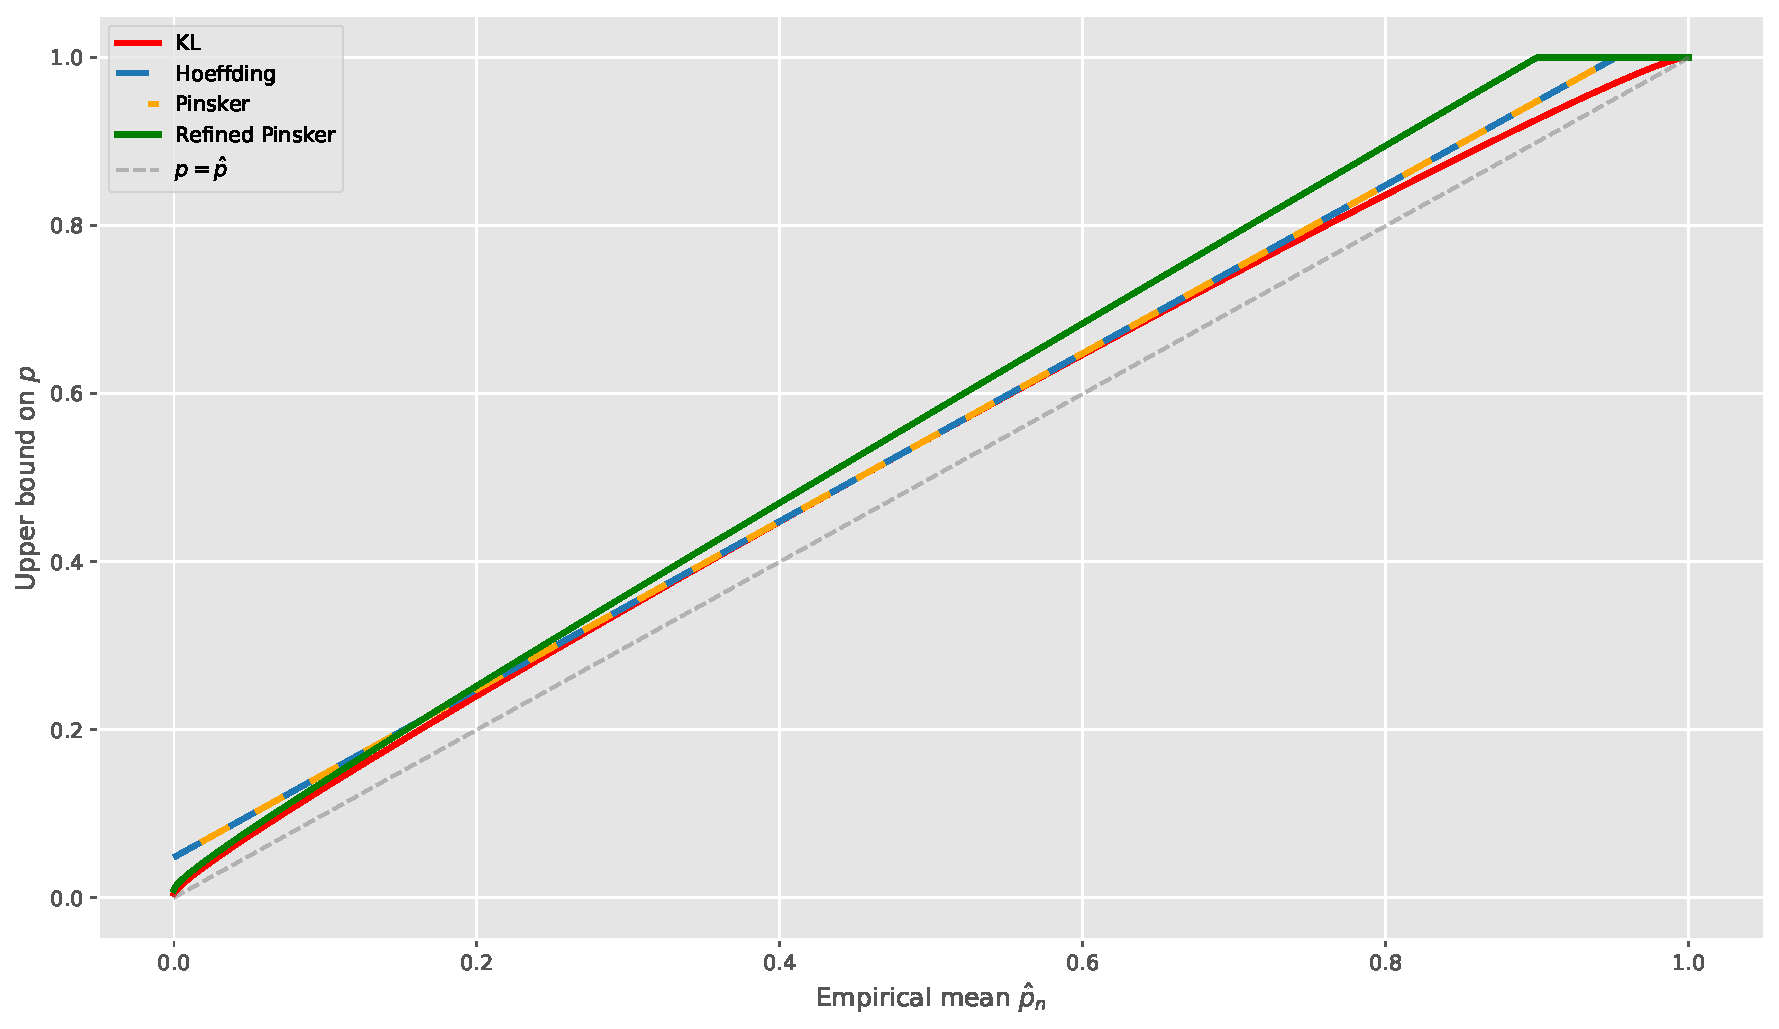
\includegraphics[scale=0.53]{figures/upper_bounds.pdf}
        \caption{Upper bounds for $\hat{p}_n \in [0,1]$}
        \label{fig:upper_bounds}
    \end{figure}
\end{center}
and in figure \ref{fig:zoomed_upper_bounds} we plot the same upper bounds "zoomed in" on $\hat{p}_n \in [0,0.1]$.
\begin{center}
    \begin{figure}[ht]
        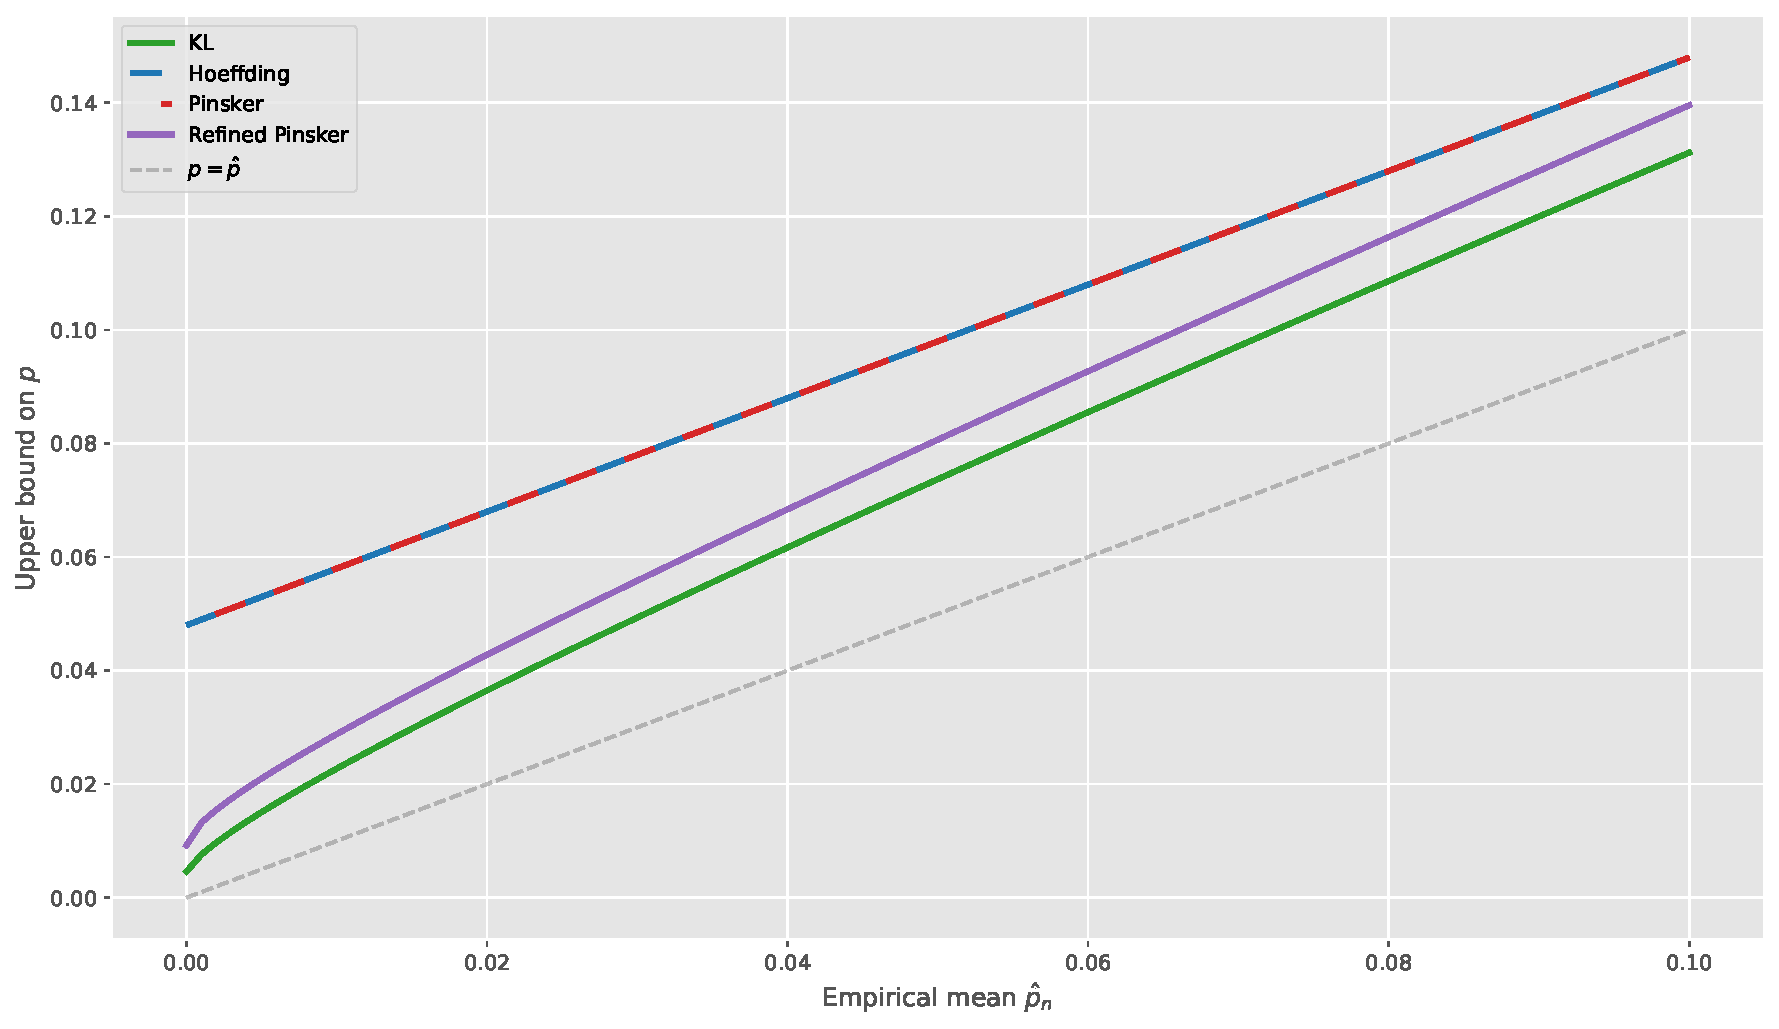
\includegraphics[scale=0.53]{figures/zoomed_in_upper_bounds.pdf}
        \caption{Zoomed upper bounds for $\hat{p}_n \in [0,0.1]$}
        \label{fig:zoomed_upper_bounds}
    \end{figure}
\end{center}

\subsection*{Plot of lower bounds}
The lower bounds are shown in figure \ref{fig:lower_bounds}.
\begin{center}
    \begin{figure}[ht]
        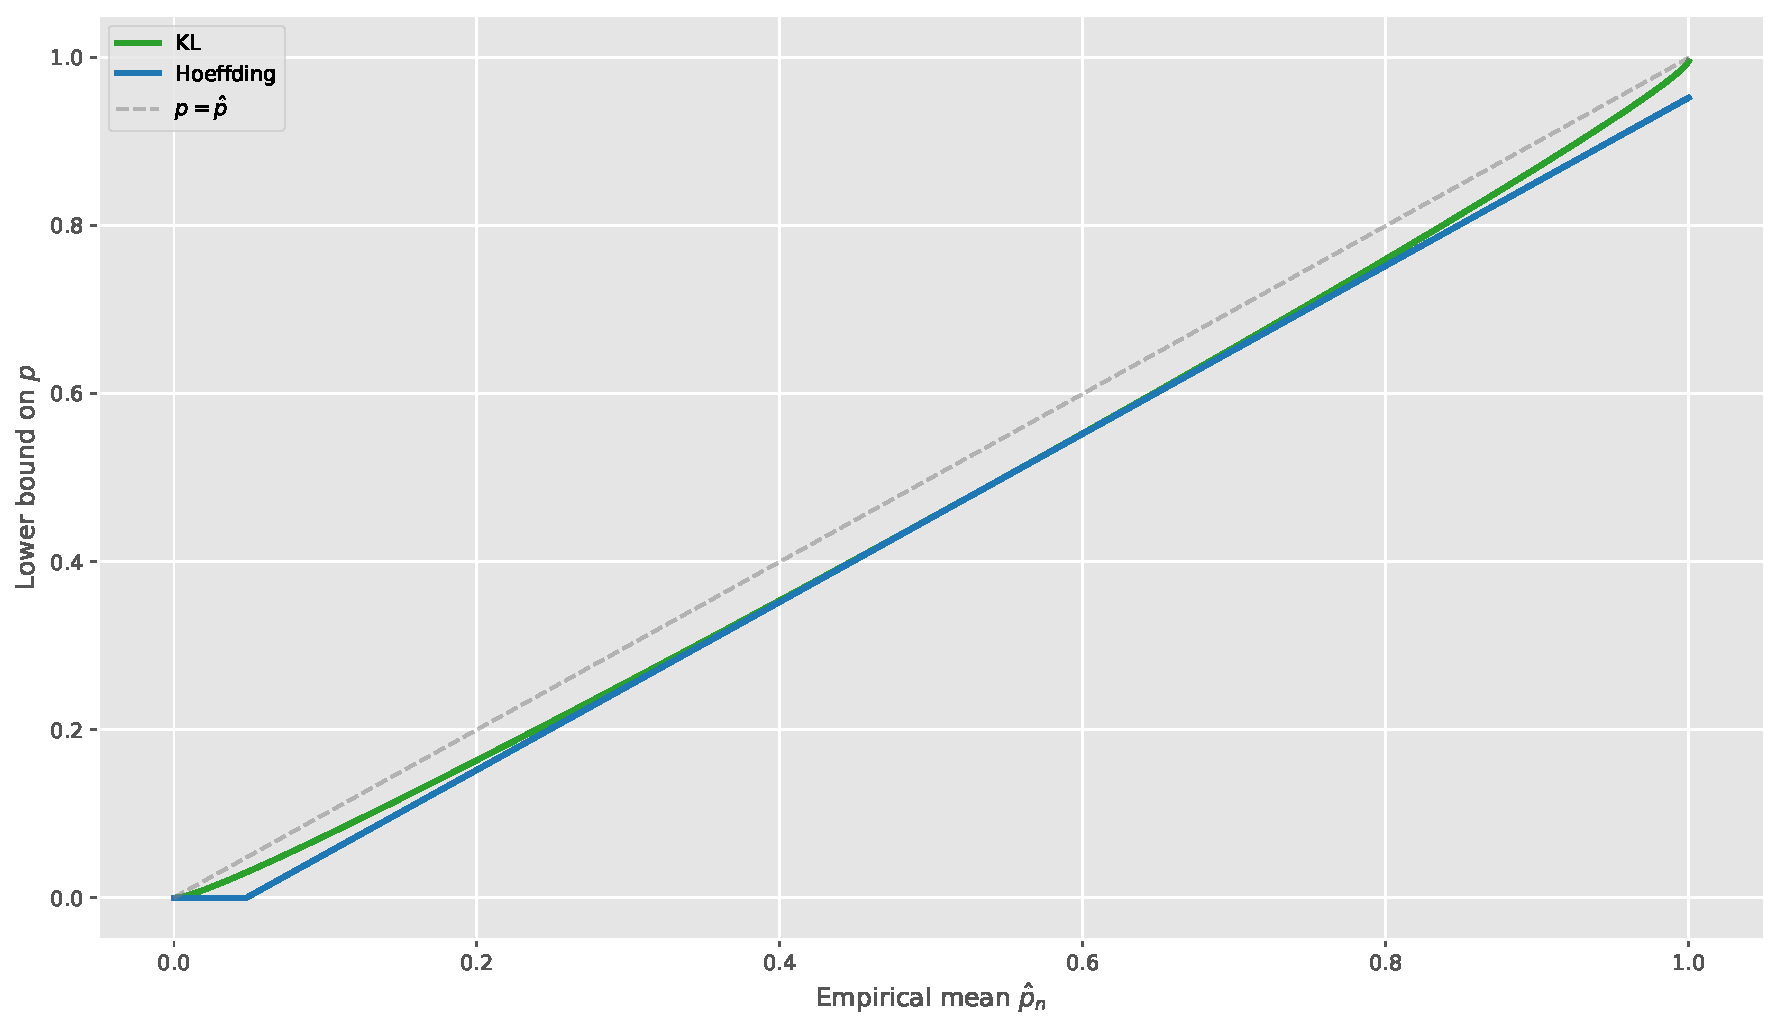
\includegraphics[scale=0.53]{figures/lower_bounds.pdf}
        \caption{Lower bounds for $\hat{p}_n \in [0,1]$}
        \label{fig:lower_bounds}
    \end{figure}
\end{center}

\subsection*{Computation of upper and lower inverse of $\kl$}
Please see \ref{lst:upper_inverse} for the implementation of the upper inverse of $\kl$. To compute the lower inverse of $\kl$, we note that $\kl(a\|b)=\kl(1-a\|1-b)$ for all $a,b \in [0,1]$. So $\kl(\hat{p}\|p) \leq \epsilon$ is equivalent to $\kl(1-\hat{p}\|1-p) \leq \epsilon$. For $q=1-p$ the sets ${p : \kl(\hat{p}\|p) \leq \epsilon}$ and ${q : \kl(1-\hat{p}\|q) \leq \epsilon}$ are identical.
\\[2mm]
By the definition of the upper inverse we have 
\begin{equation*}
    q^+ = \kl^{-1^+} (1-\hat{p}, \epsilon) = \max \{q \geq 1-\hat{p} : \kl(1-\hat{p}\|q) \leq \epsilon \}
\end{equation*}
We now replace $q$ with $1-p$ to obtain
\begin{equation*}
    p^- = 1-q^+ = 1-  \kl^{-1^+} (1-\hat{p}, \epsilon) = \min \{p \leq \hat{p}  : \kl(\hat{p}\|p) \leq \epsilon \} = \kl^{-1^-}(\hat{p}, \epsilon )
\end{equation*}
So the lower inverse can be obtained from the upper inverse through the code:
\lstinputlisting[caption=Lower inverse, label={lst:lower_inverse}, language=python, style=myStyle]{code/lower_inverse.py}

I also implemented the lower inverse using the same numerical approach as for the upper inverse and used property testing to verify that the two approaches produce same results.

\subsection*{Conclusion}
$\kl$ is the tightest bound in the whole interval $[0, 1]$. As long as we are close to $0$, refined Pinsker is only slightly worse than $\kl$. Once we pass approximately $\hat{p}_n=0.2$ Hoeffding is actually better than Refined Pinsker.